% Options for packages loaded elsewhere
\PassOptionsToPackage{unicode}{hyperref}
\PassOptionsToPackage{hyphens}{url}
%
\documentclass[
]{article}
\usepackage{amsmath,amssymb}
\usepackage{iftex}
\ifPDFTeX
  \usepackage[T1]{fontenc}
  \usepackage[utf8]{inputenc}
  \usepackage{textcomp} % provide euro and other symbols
\else % if luatex or xetex
  \usepackage{unicode-math} % this also loads fontspec
  \defaultfontfeatures{Scale=MatchLowercase}
  \defaultfontfeatures[\rmfamily]{Ligatures=TeX,Scale=1}
\fi
\usepackage{lmodern}
\ifPDFTeX\else
  % xetex/luatex font selection
\fi
% Use upquote if available, for straight quotes in verbatim environments
\IfFileExists{upquote.sty}{\usepackage{upquote}}{}
\IfFileExists{microtype.sty}{% use microtype if available
  \usepackage[]{microtype}
  \UseMicrotypeSet[protrusion]{basicmath} % disable protrusion for tt fonts
}{}
\makeatletter
\@ifundefined{KOMAClassName}{% if non-KOMA class
  \IfFileExists{parskip.sty}{%
    \usepackage{parskip}
  }{% else
    \setlength{\parindent}{0pt}
    \setlength{\parskip}{6pt plus 2pt minus 1pt}}
}{% if KOMA class
  \KOMAoptions{parskip=half}}
\makeatother
\usepackage{xcolor}
\usepackage[margin=1in]{geometry}
\usepackage{longtable,booktabs,array}
\usepackage{calc} % for calculating minipage widths
% Correct order of tables after \paragraph or \subparagraph
\usepackage{etoolbox}
\makeatletter
\patchcmd\longtable{\par}{\if@noskipsec\mbox{}\fi\par}{}{}
\makeatother
% Allow footnotes in longtable head/foot
\IfFileExists{footnotehyper.sty}{\usepackage{footnotehyper}}{\usepackage{footnote}}
\makesavenoteenv{longtable}
\usepackage{graphicx}
\makeatletter
\def\maxwidth{\ifdim\Gin@nat@width>\linewidth\linewidth\else\Gin@nat@width\fi}
\def\maxheight{\ifdim\Gin@nat@height>\textheight\textheight\else\Gin@nat@height\fi}
\makeatother
% Scale images if necessary, so that they will not overflow the page
% margins by default, and it is still possible to overwrite the defaults
% using explicit options in \includegraphics[width, height, ...]{}
\setkeys{Gin}{width=\maxwidth,height=\maxheight,keepaspectratio}
% Set default figure placement to htbp
\makeatletter
\def\fps@figure{htbp}
\makeatother
\setlength{\emergencystretch}{3em} % prevent overfull lines
\providecommand{\tightlist}{%
  \setlength{\itemsep}{0pt}\setlength{\parskip}{0pt}}
\setcounter{secnumdepth}{-\maxdimen} % remove section numbering
\ifLuaTeX
  \usepackage{selnolig}  % disable illegal ligatures
\fi
\IfFileExists{bookmark.sty}{\usepackage{bookmark}}{\usepackage{hyperref}}
\IfFileExists{xurl.sty}{\usepackage{xurl}}{} % add URL line breaks if available
\urlstyle{same}
\hypersetup{
  pdftitle={HW 2},
  pdfauthor={Denys Osmak},
  hidelinks,
  pdfcreator={LaTeX via pandoc}}

\title{HW 2}
\author{Denys Osmak}
\date{2024-01-25}

\begin{document}
\maketitle

\hypertarget{github-link}{%
\section{Github link:}\label{github-link}}

\url{https://github.com/DenysUkr/SDS-315-GitHub-Repo/tree/main/Homework/HW\%202}

\hypertarget{problem-1}{%
\section{Problem 1}\label{problem-1}}

\hypertarget{part-a}{%
\subsection{Part A}\label{part-a}}

\includegraphics{HW2--2-_files/figure-latex/unnamed-chunk-3-1.pdf}

We can tell from this graph that the largest majarity of the professors
are evaluated at around the 4/5 mark. While no professors are marked to
be 2/5 and bellow.

\hypertarget{part-b}{%
\subsection{Part B}\label{part-b}}

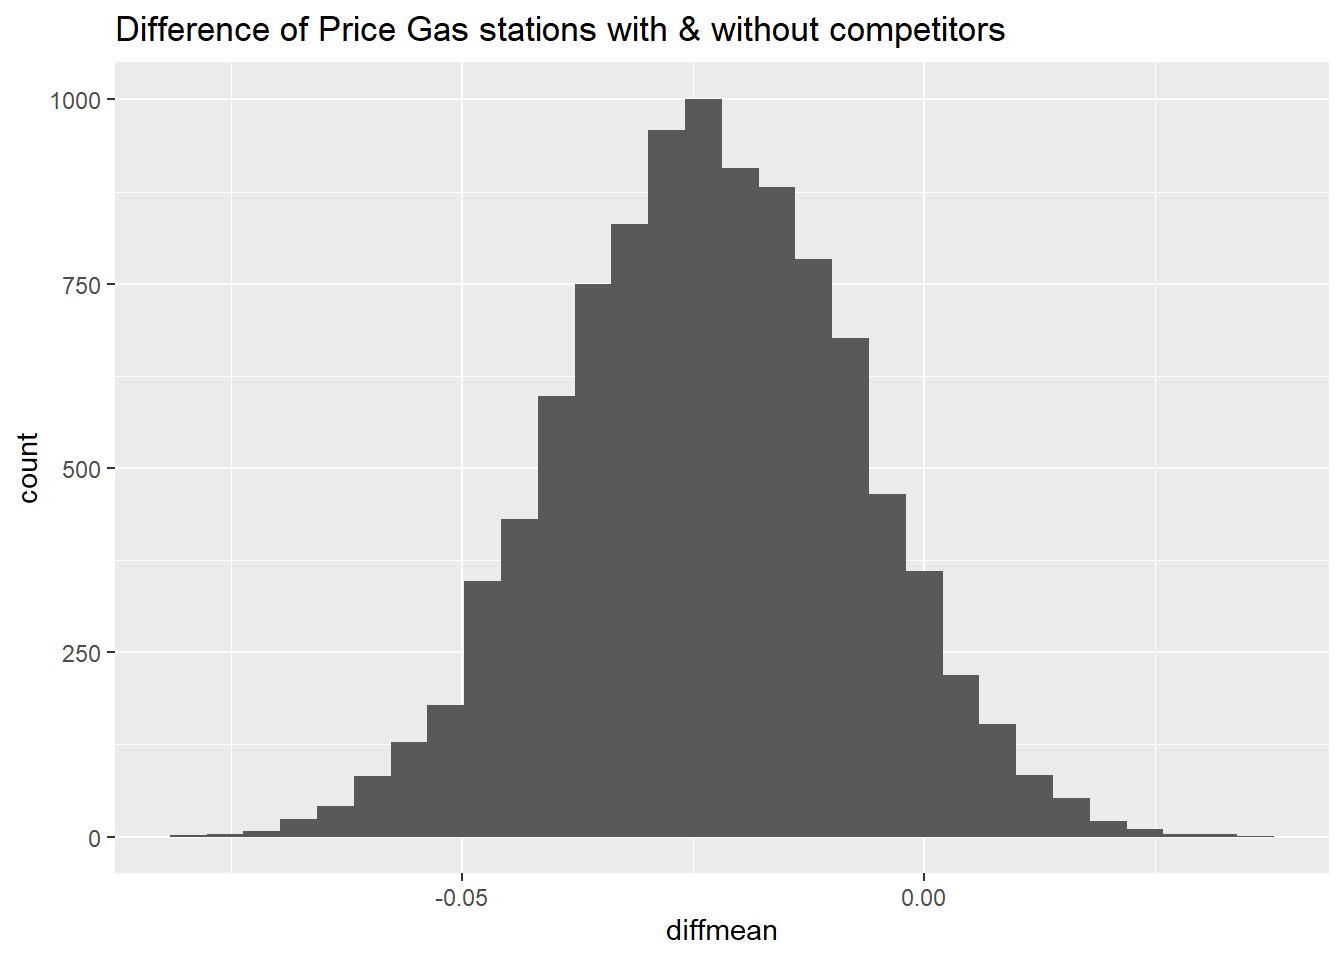
\includegraphics{HW2--2-_files/figure-latex/unnamed-chunk-4-1.pdf}

This box plot shows that there is a significant difference in evaluation
scores between professors that are native English speakers vs that are
not. From the graph we can see that on avarage a native English speaking
professor gets \textasciitilde{} 0.5 higher score then a non native
English speaker.

\hypertarget{part-c}{%
\subsection{Part C}\label{part-c}}

\includegraphics{HW2--2-_files/figure-latex/unnamed-chunk-5-1.pdf}

Due to the fact that there seems to be a larger number of male
professors, to see the true difference in the distribution of the
evaluation score between male and female professors, the charts were
normalized. After normalizing the charts it can be seen that while the
male and female professors have relativly same evaluation scores, most
of them being between 3.5-4.5, there is an abnormal ammount of female
professors that are rated 3.5 and male professors at 4.5.

\hypertarget{part-d}{%
\subsection{Part D}\label{part-d}}

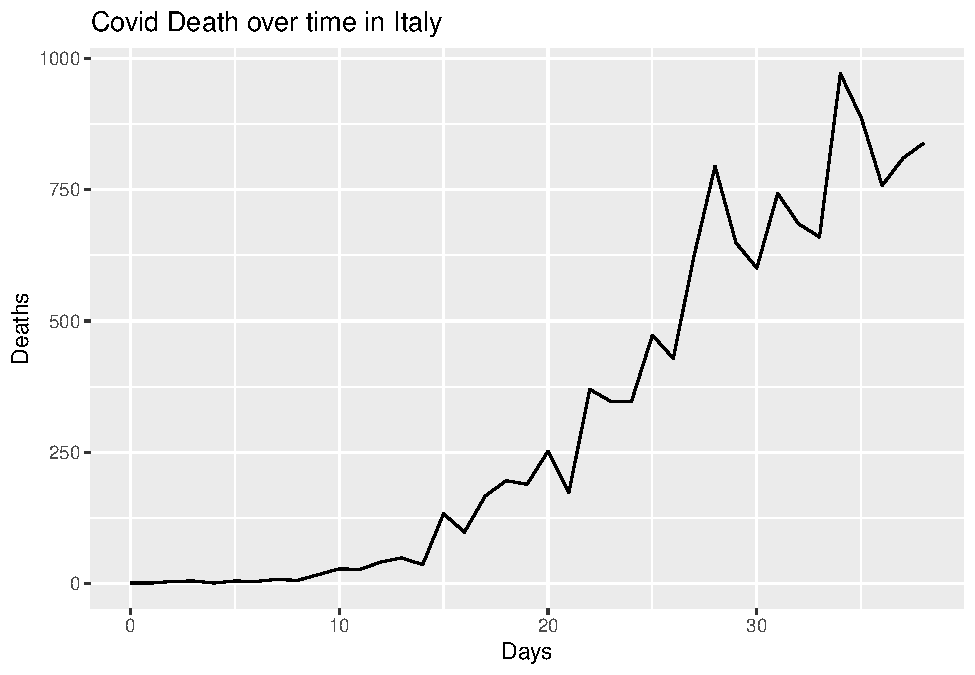
\includegraphics{HW2--2-_files/figure-latex/unnamed-chunk-6-1.pdf}

From the scatter plot there seems to be little to no correlation between
beauty score and the evaluation score.

\hypertarget{problem-2}{%
\section{Problem 2}\label{problem-2}}

\hypertarget{part-a-1}{%
\subsection{Part A}\label{part-a-1}}

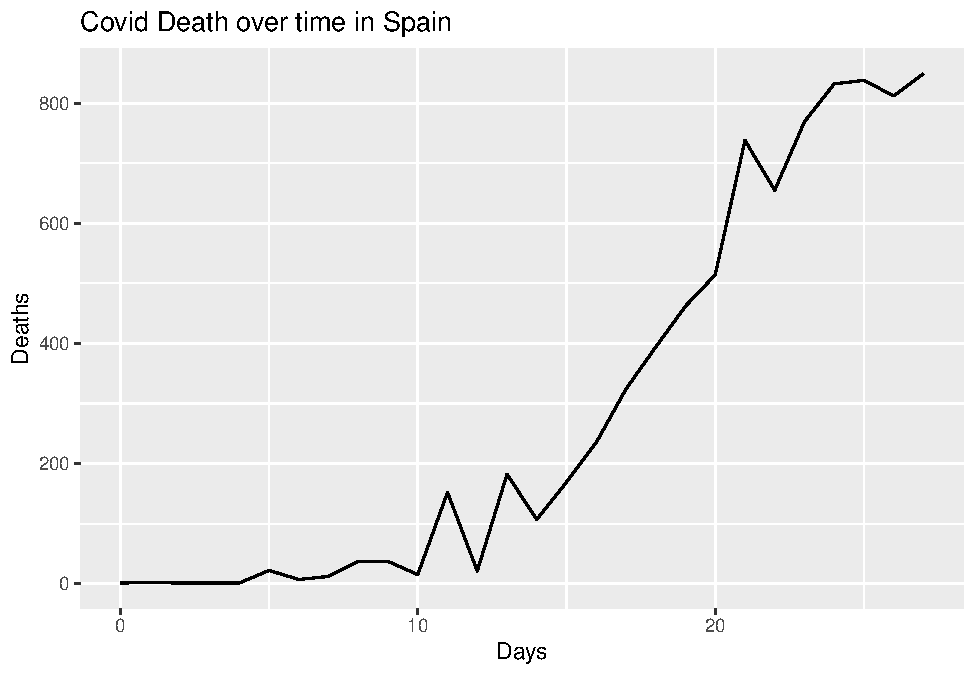
\includegraphics{HW2--2-_files/figure-latex/unnamed-chunk-7-1.pdf}

By looking at this graph we can conclude that there is a large spike of
bike rantals during the rush hours around 7 am and 6pm when people are
commuting to and from work.

\hypertarget{part-b-1}{%
\subsection{Part B}\label{part-b-1}}

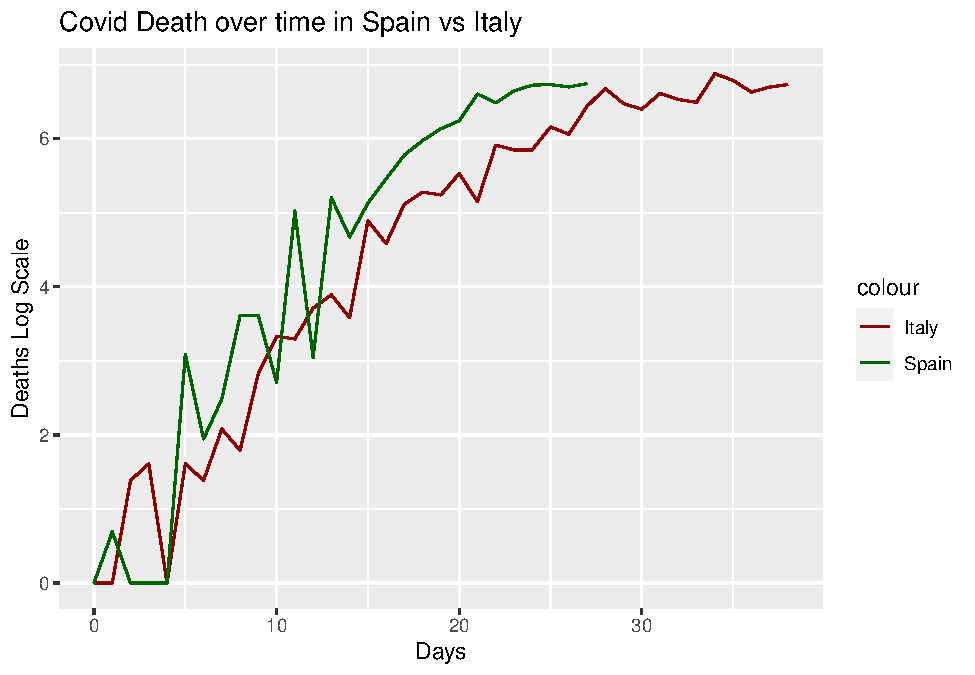
\includegraphics{HW2--2-_files/figure-latex/unnamed-chunk-8-1.pdf}

From the graph we can see that the weekends (identefied as 0) have a
much more relaxed curve. This is due to the fact that during the weeked
the bikes are used for pleasure rather then for commuting to work.

\hypertarget{part-c-1}{%
\subsection{Part C}\label{part-c-1}}

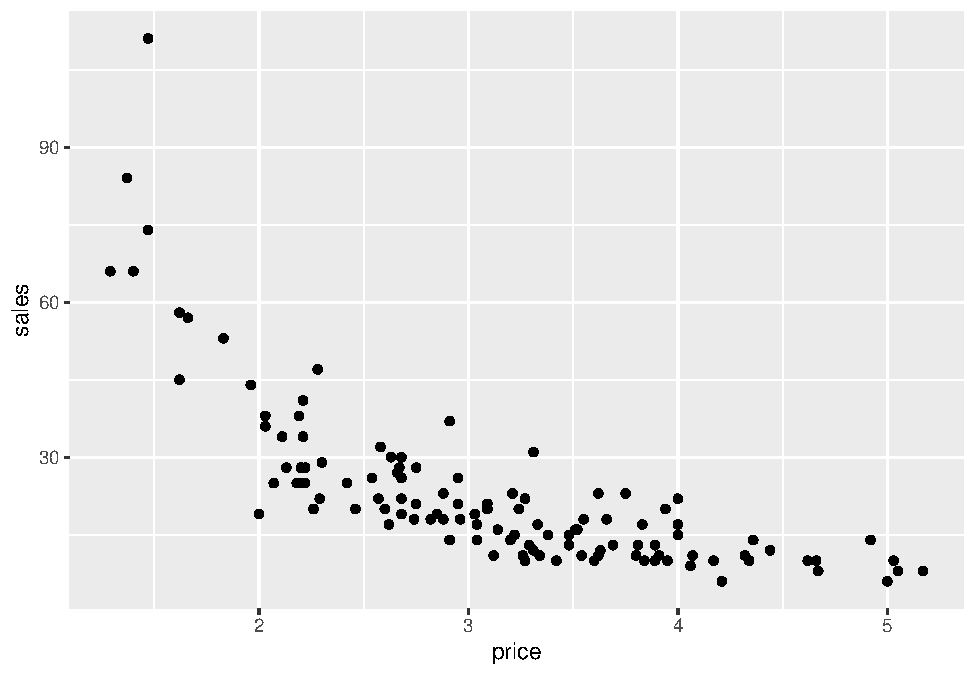
\includegraphics{HW2--2-_files/figure-latex/unnamed-chunk-9-1.pdf}

We can see that the average ridership goes down when the weather is
cloudy or has light rain ( type 2 \& 3 weather codes). Additionally
there is no recorded ridership at 9am during heavy rains.

\hypertarget{problem-3}{%
\section{Problem 3}\label{problem-3}}

\hypertarget{part-a-2}{%
\subsection{Part A}\label{part-a-2}}

\includegraphics{HW2--2-_files/figure-latex/unnamed-chunk-10-1.pdf}

By looking at the graphs, we can tell that there is the peak for
boarding for weekdays are around 3-6pm. The weekdays have very similar
curves, no matter the day of the week possibly attributed because the
buses are primary used by work commuters. Additional, the reason that
November might have the lowest is because it is the coldest month.
However the reason why September might have the lowest boarding on
Mondays might be due to the fact that there was some sort of holiday on
Monday of September of 2018, which lowered the avarage hourly boarding.

\hypertarget{part-b-2}{%
\subsection{Part B}\label{part-b-2}}

\includegraphics{HW2--2-_files/figure-latex/unnamed-chunk-11-1.pdf}

There is little to no correlation between the temperature and the
transit usage, since there is a completely vertical slope as shown on
the graph. Interesting enough the weekends tend to have less ovaral
boarding.

\hypertarget{problem-4}{%
\section{Problem 4}\label{problem-4}}

\hypertarget{part-a-3}{%
\subsection{Part A}\label{part-a-3}}

\begin{longtable}[]{@{}
  >{\raggedright\arraybackslash}p{(\columnwidth - 4\tabcolsep) * \real{0.4719}}
  >{\raggedright\arraybackslash}p{(\columnwidth - 4\tabcolsep) * \real{0.4045}}
  >{\raggedleft\arraybackslash}p{(\columnwidth - 4\tabcolsep) * \real{0.1236}}@{}}
\caption{Top Songs}\tabularnewline
\toprule\noalign{}
\begin{minipage}[b]{\linewidth}\raggedright
performer
\end{minipage} & \begin{minipage}[b]{\linewidth}\raggedright
song
\end{minipage} & \begin{minipage}[b]{\linewidth}\raggedleft
totalWeeks
\end{minipage} \\
\midrule\noalign{}
\endfirsthead
\toprule\noalign{}
\begin{minipage}[b]{\linewidth}\raggedright
performer
\end{minipage} & \begin{minipage}[b]{\linewidth}\raggedright
song
\end{minipage} & \begin{minipage}[b]{\linewidth}\raggedleft
totalWeeks
\end{minipage} \\
\midrule\noalign{}
\endhead
\bottomrule\noalign{}
\endlastfoot
Imagine Dragons & Radioactive & 87 \\
AWOLNATION & Sail & 79 \\
Jason Mraz & I'm Yours & 76 \\
The Weeknd & Blinding Lights & 76 \\
LeAnn Rimes & How Do I Live & 69 \\
LMFAO Featuring Lauren Bennett \& GoonRock & Party Rock Anthem & 68 \\
OneRepublic & Counting Stars & 68 \\
Adele & Rolling In The Deep & 65 \\
Jewel & Foolish Games/You Were Meant For Me & 65 \\
Carrie Underwood & Before He Cheats & 64 \\
\end{longtable}

\hypertarget{part-b-3}{%
\subsection{Part B}\label{part-b-3}}

\includegraphics{HW2--2-_files/figure-latex/unnamed-chunk-13-1.pdf}

There is an interesting dip how number of unique songs have doped
significantly from 1960 to 2000 and then rapidly picked back up after
2000. This might be to the fact of a music monopoly or some other
extreme factor

\hypertarget{part-c-2}{%
\subsection{Part C}\label{part-c-2}}

Let's define a ``ten-week hit'' as a single song that appeared on the
Billboard Top 100 for at least ten weeks. There are 19 artists in U.S.
musical history since 1958 who have had at least 30 songs that were
``ten-week hits.'' Make a bar plot for these 19 artists, showing how
many ten-week hits each one had in their musical career. Give the plot
an informative caption in which you explain what is shown

\hypertarget{section}{%
\subsection{}\label{section}}

\end{document}
